\documentclass[a4paper]{article}

\def\npart{III}
\def\nterm {Lent}
\def\nyear {2017-2018}
\def\nlecturer {Brian}
\def\ncourse {Decision}

\makeatletter
\ifx \nauthor\undefined
  \def\nauthor{Dexter Chua}
\else
\fi

\author{Based on lectures by \nlecturer \\\small Notes taken by \nauthor}
\date{\nterm\ \nyear}

\usepackage{alltt}
\usepackage{amsfonts}
\usepackage{amsmath}
\usepackage{amssymb}
\usepackage{amsthm}
\usepackage{booktabs}
\usepackage{caption}
\usepackage{enumitem}
\usepackage{fancyhdr}
\usepackage{graphicx}
\usepackage{mathdots}
\usepackage{mathtools}
\usepackage{microtype}
\usepackage{multirow}
\usepackage{pdflscape}
\usepackage{pgfplots}
\usepackage{siunitx}
\usepackage{slashed}
\usepackage{tabularx}
\usepackage{tikz}
\usepackage{tkz-euclide}
\usepackage[normalem]{ulem}
\usepackage[all]{xy}
\usepackage{imakeidx}

\makeindex[intoc, title=Index]
\indexsetup{othercode={\lhead{\emph{Index}}}}

\ifx \nextra \undefined
  \usepackage[pdftex,
    hidelinks,
    pdfauthor={Dexter Chua},
    pdfsubject={Cambridge Maths Notes: Part \npart\ - \ncourse},
    pdftitle={Part \npart\ - \ncourse},
  pdfkeywords={Cambridge Mathematics Maths Math \npart\ \nterm\ \nyear\ \ncourse}]{hyperref}
  \title{Part \npart\ --- \ncourse}
\else
  \usepackage[pdftex,
    hidelinks,
    pdfauthor={Dexter Chua},
    pdfsubject={Cambridge Maths Notes: Part \npart\ - \ncourse\ (\nextra)},
    pdftitle={Part \npart\ - \ncourse\ (\nextra)},
  pdfkeywords={Cambridge Mathematics Maths Math \npart\ \nterm\ \nyear\ \ncourse\ \nextra}]{hyperref}

  \title{Part \npart\ --- \ncourse \\ {\Large \nextra}}
  \renewcommand\printindex{}
\fi

\pgfplotsset{compat=1.12}

\pagestyle{fancyplain}
\ifx \ncoursehead \undefined
\def\ncoursehead{\ncourse}
\fi

\lhead{\emph{\nouppercase{\leftmark}}}
\ifx \nextra \undefined
  \rhead{
    \ifnum\thepage=1
    \else
      \npart\ \ncoursehead
    \fi}
\else
  \rhead{
    \ifnum\thepage=1
    \else
      \npart\ \ncoursehead \ (\nextra)
    \fi}
\fi
\usetikzlibrary{arrows.meta}
\usetikzlibrary{decorations.markings}
\usetikzlibrary{decorations.pathmorphing}
\usetikzlibrary{positioning}
\usetikzlibrary{fadings}
\usetikzlibrary{intersections}
\usetikzlibrary{cd}

\newcommand*{\Cdot}{{\raisebox{-0.25ex}{\scalebox{1.5}{$\cdot$}}}}
\newcommand {\pd}[2][ ]{
  \ifx #1 { }
    \frac{\partial}{\partial #2}
  \else
    \frac{\partial^{#1}}{\partial #2^{#1}}
  \fi
}
\ifx \nhtml \undefined
\else
  \renewcommand\printindex{}
  \DisableLigatures[f]{family = *}
  \let\Contentsline\contentsline
  \renewcommand\contentsline[3]{\Contentsline{#1}{#2}{}}
  \renewcommand{\@dotsep}{10000}
  \newlength\currentparindent
  \setlength\currentparindent\parindent

  \newcommand\@minipagerestore{\setlength{\parindent}{\currentparindent}}
  \usepackage[active,tightpage,pdftex]{preview}
  \renewcommand{\PreviewBorder}{0.1cm}

  \newenvironment{stretchpage}%
  {\begin{preview}\begin{minipage}{\hsize}}%
    {\end{minipage}\end{preview}}
  \AtBeginDocument{\begin{stretchpage}}
  \AtEndDocument{\end{stretchpage}}

  \newcommand{\@@newpage}{\end{stretchpage}\begin{stretchpage}}

  \let\@real@section\section
  \renewcommand{\section}{\@@newpage\@real@section}
  \let\@real@subsection\subsection
  \renewcommand{\subsection}{\@ifstar{\@real@subsection*}{\@@newpage\@real@subsection}}
\fi
\ifx \ntrim \undefined
\else
  \usepackage{geometry}
  \geometry{
    papersize={379pt, 699pt},
    textwidth=345pt,
    textheight=596pt,
    left=17pt,
    top=54pt,
    right=17pt
  }
\fi

\ifx \nisofficial \undefined
\let\@real@maketitle\maketitle
\renewcommand{\maketitle}{\@real@maketitle\begin{center}\begin{minipage}[c]{0.9\textwidth}\centering\footnotesize These notes are not endorsed by the lecturers, and I have modified them (often significantly) after lectures. They are nowhere near accurate representations of what was actually lectured, and in particular, all errors are almost surely mine.\end{minipage}\end{center}}
\else
\fi

% Theorems
\theoremstyle{definition}
\newtheorem*{aim}{Aim}
\newtheorem*{axiom}{Axiom}
\newtheorem*{claim}{Claim}
\newtheorem*{cor}{Corollary}
\newtheorem*{conjecture}{Conjecture}
\newtheorem*{defi}{Definition}
\newtheorem*{eg}{Example}
\newtheorem*{ex}{Exercise}
\newtheorem*{fact}{Fact}
\newtheorem*{law}{Law}
\newtheorem*{lemma}{Lemma}
\newtheorem*{notation}{Notation}
\newtheorem*{prop}{Proposition}
\newtheorem*{question}{Question}
\newtheorem*{rrule}{Rule}
\newtheorem*{thm}{Theorem}
\newtheorem*{assumption}{Assumption}

\newtheorem*{remark}{Remark}
\newtheorem*{warning}{Warning}
\newtheorem*{exercise}{Exercise}

\newtheorem{nthm}{Theorem}[section]
\newtheorem{nlemma}[nthm]{Lemma}
\newtheorem{nprop}[nthm]{Proposition}
\newtheorem{ncor}[nthm]{Corollary}


\renewcommand{\labelitemi}{--}
\renewcommand{\labelitemii}{$\circ$}
\renewcommand{\labelenumi}{(\roman{*})}

\let\stdsection\section
\renewcommand\section{\newpage\stdsection}

\newcommand\qedsym{\hfill\ensuremath{\square}}
% Strike through
\def\st{\bgroup \ULdepth=-.55ex \ULset}


%%%%%%%%%%%%%%%%%%%%%%%%%
%%%%% Maths Symbols %%%%%
%%%%%%%%%%%%%%%%%%%%%%%%%

% Matrix groups
\newcommand{\GL}{\mathrm{GL}}
\newcommand{\Or}{\mathrm{O}}
\newcommand{\PGL}{\mathrm{PGL}}
\newcommand{\PSL}{\mathrm{PSL}}
\newcommand{\PSO}{\mathrm{PSO}}
\newcommand{\PSU}{\mathrm{PSU}}
\newcommand{\SL}{\mathrm{SL}}
\newcommand{\SO}{\mathrm{SO}}
\newcommand{\Spin}{\mathrm{Spin}}
\newcommand{\Sp}{\mathrm{Sp}}
\newcommand{\SU}{\mathrm{SU}}
\newcommand{\U}{\mathrm{U}}
\newcommand{\Mat}{\mathrm{Mat}}

% Matrix algebras
\newcommand{\gl}{\mathfrak{gl}}
\newcommand{\ort}{\mathfrak{o}}
\newcommand{\so}{\mathfrak{so}}
\newcommand{\su}{\mathfrak{su}}
\newcommand{\uu}{\mathfrak{u}}
\renewcommand{\sl}{\mathfrak{sl}}

% Special sets
\newcommand{\C}{\mathbb{C}}
\newcommand{\CP}{\mathbb{CP}}
\newcommand{\GG}{\mathbb{G}}
\newcommand{\N}{\mathbb{N}}
\newcommand{\Q}{\mathbb{Q}}
\newcommand{\R}{\mathbb{R}}
\newcommand{\RP}{\mathbb{RP}}
\newcommand{\T}{\mathbb{T}}
\newcommand{\Z}{\mathbb{Z}}
\renewcommand{\H}{\mathbb{H}}

% Brackets
\newcommand{\abs}[1]{\left\lvert #1\right\rvert}
\newcommand{\bket}[1]{\left\lvert #1\right\rangle}
\newcommand{\brak}[1]{\left\langle #1 \right\rvert}
\newcommand{\braket}[2]{\left\langle #1\middle\vert #2 \right\rangle}
\newcommand{\bra}{\langle}
\newcommand{\ket}{\rangle}
\newcommand{\norm}[1]{\left\lVert #1\right\rVert}
\newcommand{\normalorder}[1]{\mathop{:}\nolimits\!#1\!\mathop{:}\nolimits}
\newcommand{\tv}[1]{|#1|}
\renewcommand{\vec}[1]{\boldsymbol{\mathbf{#1}}}

% not-math
\newcommand{\bolds}[1]{{\bfseries #1}}
\newcommand{\cat}[1]{\mathsf{#1}}
\newcommand{\ph}{\,\cdot\,}
\newcommand{\term}[1]{\emph{#1}\index{#1}}
\newcommand{\phantomeq}{\hphantom{{}={}}}
% Probability
\DeclareMathOperator{\Bernoulli}{Bernoulli}
\DeclareMathOperator{\betaD}{beta}
\DeclareMathOperator{\bias}{bias}
\DeclareMathOperator{\binomial}{binomial}
\DeclareMathOperator{\corr}{corr}
\DeclareMathOperator{\cov}{cov}
\DeclareMathOperator{\gammaD}{gamma}
\DeclareMathOperator{\mse}{mse}
\DeclareMathOperator{\multinomial}{multinomial}
\DeclareMathOperator{\Poisson}{Poisson}
\DeclareMathOperator{\var}{var}
\newcommand{\E}{\mathbb{E}}
\newcommand{\Prob}{\mathbb{P}}

% Algebra
\DeclareMathOperator{\adj}{adj}
\DeclareMathOperator{\Ann}{Ann}
\DeclareMathOperator{\Aut}{Aut}
\DeclareMathOperator{\Char}{char}
\DeclareMathOperator{\disc}{disc}
\DeclareMathOperator{\dom}{dom}
\DeclareMathOperator{\fix}{fix}
\DeclareMathOperator{\Hom}{Hom}
\DeclareMathOperator{\id}{id}
\DeclareMathOperator{\image}{image}
\DeclareMathOperator{\im}{im}
\DeclareMathOperator{\tr}{tr}
\DeclareMathOperator{\Tr}{Tr}
\newcommand{\Bilin}{\mathrm{Bilin}}
\newcommand{\Frob}{\mathrm{Frob}}

% Others
\newcommand\ad{\mathrm{ad}}
\newcommand\Art{\mathrm{Art}}
\newcommand{\B}{\mathcal{B}}
\newcommand{\cU}{\mathcal{U}}
\newcommand{\Der}{\mathrm{Der}}
\newcommand{\D}{\mathrm{D}}
\newcommand{\dR}{\mathrm{dR}}
\newcommand{\exterior}{\mathchoice{{\textstyle\bigwedge}}{{\bigwedge}}{{\textstyle\wedge}}{{\scriptstyle\wedge}}}
\newcommand{\F}{\mathbb{F}}
\newcommand{\G}{\mathcal{G}}
\newcommand{\Gr}{\mathrm{Gr}}
\newcommand{\haut}{\mathrm{ht}}
\newcommand{\Hol}{\mathrm{Hol}}
\newcommand{\hol}{\mathfrak{hol}}
\newcommand{\Id}{\mathrm{Id}}
\newcommand{\lie}[1]{\mathfrak{#1}}
\newcommand{\op}{\mathrm{op}}
\newcommand{\Oc}{\mathcal{O}}
\newcommand{\pr}{\mathrm{pr}}
\newcommand{\Ps}{\mathcal{P}}
\newcommand{\pt}{\mathrm{pt}}
\newcommand{\qeq}{\mathrel{``{=}"}}
\newcommand{\Rs}{\mathcal{R}}
\newcommand{\Vect}{\mathrm{Vect}}
\newcommand{\wsto}{\stackrel{\mathrm{w}^*}{\to}}
\newcommand{\wt}{\mathrm{wt}}
\newcommand{\wto}{\stackrel{\mathrm{w}}{\to}}
\renewcommand{\d}{\mathrm{d}}
\renewcommand{\P}{\mathbb{P}}
%\renewcommand{\F}{\mathcal{F}}


\let\Im\relax
\let\Re\relax

\DeclareMathOperator{\area}{area}
\DeclareMathOperator{\card}{card}
\DeclareMathOperator{\ccl}{ccl}
\DeclareMathOperator{\ch}{ch}
\DeclareMathOperator{\cl}{cl}
\DeclareMathOperator{\cls}{\overline{\mathrm{span}}}
\DeclareMathOperator{\coker}{coker}
\DeclareMathOperator{\conv}{conv}
\DeclareMathOperator{\cosec}{cosec}
\DeclareMathOperator{\cosech}{cosech}
\DeclareMathOperator{\covol}{covol}
\DeclareMathOperator{\diag}{diag}
\DeclareMathOperator{\diam}{diam}
\DeclareMathOperator{\Diff}{Diff}
\DeclareMathOperator{\End}{End}
\DeclareMathOperator{\energy}{energy}
\DeclareMathOperator{\erfc}{erfc}
\DeclareMathOperator{\erf}{erf}
\DeclareMathOperator*{\esssup}{ess\,sup}
\DeclareMathOperator{\ev}{ev}
\DeclareMathOperator{\Ext}{Ext}
\DeclareMathOperator{\fst}{fst}
\DeclareMathOperator{\Fit}{Fit}
\DeclareMathOperator{\Frac}{Frac}
\DeclareMathOperator{\Gal}{Gal}
\DeclareMathOperator{\gr}{gr}
\DeclareMathOperator{\hcf}{hcf}
\DeclareMathOperator{\Im}{Im}
\DeclareMathOperator{\Ind}{Ind}
\DeclareMathOperator{\Int}{Int}
\DeclareMathOperator{\Isom}{Isom}
\DeclareMathOperator{\lcm}{lcm}
\DeclareMathOperator{\length}{length}
\DeclareMathOperator{\Lie}{Lie}
\DeclareMathOperator{\like}{like}
\DeclareMathOperator{\Lk}{Lk}
\DeclareMathOperator{\Maps}{Maps}
\DeclareMathOperator{\orb}{orb}
\DeclareMathOperator{\ord}{ord}
\DeclareMathOperator{\otp}{otp}
\DeclareMathOperator{\poly}{poly}
\DeclareMathOperator{\rank}{rank}
\DeclareMathOperator{\rel}{rel}
\DeclareMathOperator{\Rad}{Rad}
\DeclareMathOperator{\Re}{Re}
\DeclareMathOperator*{\res}{res}
\DeclareMathOperator{\Res}{Res}
\DeclareMathOperator{\Ric}{Ric}
\DeclareMathOperator{\rk}{rk}
\DeclareMathOperator{\Rees}{Rees}
\DeclareMathOperator{\Root}{Root}
\DeclareMathOperator{\sech}{sech}
\DeclareMathOperator{\sgn}{sgn}
\DeclareMathOperator{\snd}{snd}
\DeclareMathOperator{\Spec}{Spec}
\DeclareMathOperator{\spn}{span}
\DeclareMathOperator{\stab}{stab}
\DeclareMathOperator{\St}{St}
\DeclareMathOperator{\supp}{supp}
\DeclareMathOperator{\Syl}{Syl}
\DeclareMathOperator{\Sym}{Sym}
\DeclareMathOperator{\vol}{vol}

\pgfarrowsdeclarecombine{twolatex'}{twolatex'}{latex'}{latex'}{latex'}{latex'}
\tikzset{->/.style = {decoration={markings,
                                  mark=at position 1 with {\arrow[scale=2]{latex'}}},
                      postaction={decorate}}}
\tikzset{<-/.style = {decoration={markings,
                                  mark=at position 0 with {\arrowreversed[scale=2]{latex'}}},
                      postaction={decorate}}}
\tikzset{<->/.style = {decoration={markings,
                                   mark=at position 0 with {\arrowreversed[scale=2]{latex'}},
                                   mark=at position 1 with {\arrow[scale=2]{latex'}}},
                       postaction={decorate}}}
\tikzset{->-/.style = {decoration={markings,
                                   mark=at position #1 with {\arrow[scale=2]{latex'}}},
                       postaction={decorate}}}
\tikzset{-<-/.style = {decoration={markings,
                                   mark=at position #1 with {\arrowreversed[scale=2]{latex'}}},
                       postaction={decorate}}}
\tikzset{->>/.style = {decoration={markings,
                                  mark=at position 1 with {\arrow[scale=2]{latex'}}},
                      postaction={decorate}}}
\tikzset{<<-/.style = {decoration={markings,
                                  mark=at position 0 with {\arrowreversed[scale=2]{twolatex'}}},
                      postaction={decorate}}}
\tikzset{<<->>/.style = {decoration={markings,
                                   mark=at position 0 with {\arrowreversed[scale=2]{twolatex'}},
                                   mark=at position 1 with {\arrow[scale=2]{twolatex'}}},
                       postaction={decorate}}}
\tikzset{->>-/.style = {decoration={markings,
                                   mark=at position #1 with {\arrow[scale=2]{twolatex'}}},
                       postaction={decorate}}}
\tikzset{-<<-/.style = {decoration={markings,
                                   mark=at position #1 with {\arrowreversed[scale=2]{twolatex'}}},
                       postaction={decorate}}}

\tikzset{circ/.style = {fill, circle, inner sep = 0, minimum size = 3}}
\tikzset{scirc/.style = {fill, circle, inner sep = 0, minimum size = 1.5}}
\tikzset{mstate/.style={circle, draw, blue, text=black, minimum width=0.7cm}}

\tikzset{eqpic/.style={baseline={([yshift=-.5ex]current bounding box.center)}}}
\tikzset{commutative diagrams/.cd,cdmap/.style={/tikz/column 1/.append style={anchor=base east},/tikz/column 2/.append style={anchor=base west},row sep=tiny}}

\definecolor{mblue}{rgb}{0.2, 0.3, 0.8}
\definecolor{morange}{rgb}{1, 0.5, 0}
\definecolor{mgreen}{rgb}{0.1, 0.4, 0.2}
\definecolor{mred}{rgb}{0.5, 0, 0}

\def\drawcirculararc(#1,#2)(#3,#4)(#5,#6){%
    \pgfmathsetmacro\cA{(#1*#1+#2*#2-#3*#3-#4*#4)/2}%
    \pgfmathsetmacro\cB{(#1*#1+#2*#2-#5*#5-#6*#6)/2}%
    \pgfmathsetmacro\cy{(\cB*(#1-#3)-\cA*(#1-#5))/%
                        ((#2-#6)*(#1-#3)-(#2-#4)*(#1-#5))}%
    \pgfmathsetmacro\cx{(\cA-\cy*(#2-#4))/(#1-#3)}%
    \pgfmathsetmacro\cr{sqrt((#1-\cx)*(#1-\cx)+(#2-\cy)*(#2-\cy))}%
    \pgfmathsetmacro\cA{atan2(#2-\cy,#1-\cx)}%
    \pgfmathsetmacro\cB{atan2(#6-\cy,#5-\cx)}%
    \pgfmathparse{\cB<\cA}%
    \ifnum\pgfmathresult=1
        \pgfmathsetmacro\cB{\cB+360}%
    \fi
    \draw (#1,#2) arc (\cA:\cB:\cr);%
}
\newcommand\getCoord[3]{\newdimen{#1}\newdimen{#2}\pgfextractx{#1}{\pgfpointanchor{#3}{center}}\pgfextracty{#2}{\pgfpointanchor{#3}{center}}}

\newcommand\qedshift{\vspace{-17pt}}
\newcommand\fakeqed{\pushQED{\qed}\qedhere}

\def\Xint#1{\mathchoice
   {\XXint\displaystyle\textstyle{#1}}%
   {\XXint\textstyle\scriptstyle{#1}}%
   {\XXint\scriptstyle\scriptscriptstyle{#1}}%
   {\XXint\scriptscriptstyle\scriptscriptstyle{#1}}%
   \!\int}
\def\XXint#1#2#3{{\setbox0=\hbox{$#1{#2#3}{\int}$}
     \vcenter{\hbox{$#2#3$}}\kern-.5\wd0}}
\def\ddashint{\Xint=}
\def\dashint{\Xint-}

\newcommand\separator{{\centering\rule{2cm}{0.2pt}\vspace{2pt}\par}}

\newenvironment{own}{\color{gray!70!black}}{}

\newcommand\makecenter[1]{\raisebox{-0.5\height}{#1}}

\mathchardef\mdash="2D

\newenvironment{significant}{\begin{center}\begin{minipage}{0.9\textwidth}\centering\em}{\end{minipage}\end{center}}
\DeclareRobustCommand{\rvdots}{%
  \vbox{
    \baselineskip4\p@\lineskiplimit\z@
    \kern-\p@
    \hbox{.}\hbox{.}\hbox{.}
  }}
\DeclareRobustCommand\tph[3]{{\texorpdfstring{#1}{#2}}}
\makeatother

\usetikzlibrary[topaths]
\usetikzlibrary{positioning,chains,fit,shapes,calc}
% A counter, since TikZ is not clever enough (yet) to handle
% arbitrary angle systems.
\newcount\mycount
\usepackage{verbatim}



\begin{document}

\maketitle

\tableofcontents

\section{Algorithms}
\subsection{Use an algorithm given in words}
\begin{eg}
	The 'happy' algorithm is
	\begin{itemize}
		\item write down any integer
		\item square its digits and find the sum of the squares
		\item continue with this number
		      1		\item repeat until either the answer is 1 (happy) or until you get trapped in a cycle (not happy).
	\end{itemize}
	Show that
	\begin{enumerate}
		\item 70 is happy
		\item 4 is unhappy
	\end{enumerate}
	\begin{proof}
		\begin{enumerate}
			\item \begin{align*} 7^2+0^2&=49 \\ 4^2+9^2 &= 96 \\ 9^2+7^2 &= 130 \\ 1^2+3^2 + 0^2 &=10 \\1^2 +0^2 &=1 \\ \text{so 70 is happy} \end{align*}
			\item  \begin{align*} 4^2 &=16 \\ 1^2+6^2 &=37 \\ 3^2+7^2 &= 58 \\ 5^2+8^2 &= 89 \\ 1^2+4^2+5^2 &= 42 \\ 4^2+2^2 &= 20 \\ 2^2+0^2 &= 4 \\ 4^2 &=16 \\ \text{so 4 is unhappy} \end{align*}
		\end{enumerate}
	\end{proof}
\end{eg}

\begin{eg}
	Implement this algorithm
	\begin{itemize}
		\item Let $n+1,A=1,B=1$
		\item Write down A and B
		\item Let $ C=A+B$
		\item Write down C
		\item Let $n=n+1,A=B,B=C$
		\item If $n<5$ go to 3
		\item If $n=5$ stop
	\end{itemize}
	\begin{proof}
		\begin{centering}
			\begin{tabular}{|c|c|c|c|c|c|}
				\hline
				Instruction step & n & A & B & C & Write down \\
				\hline
				1                & 1 & 1 & 1 &   &            \\
				\hline
				2                &   &   &   &   & 1,1        \\
				\hline
				3                &   &   &   & 2 &            \\
				\hline
				4                &   &   &   &   & 2          \\
				\hline
				5                & 2 & 1 & 2 &   &            \\
				\hline
				6 & Go to step 3& \\
				\hline
				3                &   &   &   & 3 &            \\
				\hline
				4                &   &   &   &   & 3          \\
				\hline
				5                & 3 & 2 & 3 &   &            \\
				\hline
				6 &Go to Step 3 \\
				\hline
				3                &   &   &   & 5 &            \\
				\hline
				4                &   &   &   &   & 5          \\
				\hline
				5                & 4 & 3 & 5 &   &            \\
				\hline
				6 & Go to Step 3 \\
				\hline
				3                &   &   &   & 8 &            \\
				\hline
				4                &   &   &   &   & 8          \\
				\hline
				5                & 5 & 5 & 8 &   &            \\
				\hline
				6 &Continue to Step 7\\
				\hline
				7 & Stop\\
				\hline
			\end{tabular}
		\end{centering}
	\end{proof}
\end{eg}

\begin{eg}
	The algorithm multiplies the two numbers A and B.
	\begin{itemize}
		\item Make a table with two columns\\Write A in the top row of the left hand column and $B$ in the top row of the right hand column
		\item In the next row of the table write: \begin{itemize}\item in the left hand column, the number that is half $A$, ignoring remainders \item in the right hand column the number that is double $B$ \end{itemize}
		\item Repeat step 2 until you reach the row which has a 1 in the left hand column
		\item Delete all rows where the number in the left hand column is even
		\item Find the sum of the non-deleted numbers in the right hand column\\This is the product $AB$
	\end{itemize}
	Implement this algorithm when
	\begin{enumerate}
		\item $A=29$ and $B=34$
		\item $A=66$ and $B=56$
	\end{enumerate}
	\begin{proof}
		\begin{centering}
			\begin{enumerate}
				\item \begin{tabular}{|c|c|c|}
					      \hline
					      A     & B   & Step 4 \\
					      \hline
					      14    & 68  & Delete \\
					      \hline
					      7     & 136 &        \\
					      \hline
					      3     & 272 &        \\
					      \hline
					      1     & 544 &        \\
					      \hline
					      Total & 986 &        \\
					      \hline
				      \end{tabular}
				      So $29 \times 34 =986$
				\item \begin{tabular}{|c|c|c|}
					      \hline
					      A     & B    & Step 4 \\
					      \hline
					      66    & 56   & Delete \\
					      \hline
					      33    & 112  &        \\
					      \hline
					      16    & 224  & Delete \\
					      \hline
					      8     & 448  & Delete \\
					      \hline
					      4     & 896  & Delete \\
					      \hline
					      2     & 1792 & Delete \\
					      \hline
					      1     & 3584 &        \\
					      \hline
					      Total & 3584 &        \\
					      \hline
				      \end{tabular}
				      So $66\times56=3696$
			\end{enumerate}
		\end{centering}
	\end{proof}
\end{eg}

\subsection{Implement an algorithm given in the form of a flow chat}
There are three shapes of boxes which are used in the examination\\
\begin{centering}
	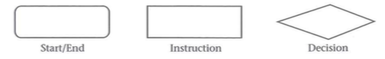
\includegraphics{img_D/2.png}
\end{centering}
\begin{eg}
	\vspace{10pt}

	\begin{enumerate}
		\item Implement this algorithm using a trace table
		\item Alter box 4 to read 'Let $E=3n$' and implement the algorithm again.
	\end{enumerate}
	How does this alter the algorithm?

	\begin{proof}

		\begin{enumerate}
			\item \begin{tabular}{|c|c|c|}
				      \hline
				      n     & E   & box 6 \\
				      \hline
				      14    & 68  & no    \\
				      \hline
				      7     & 136 & no    \\
				      \hline
				      3     & 272 & no    \\
				      \hline
				      1     & 544 & no    \\
				      \hline
				      Total & 986 & no    \\
				      \hline
			      \end{tabular}

			\item \begin{tabular}{|c|c|c|}
				      \hline
				      n     & E    & box 6 \\
				      \hline
				      66    & 56   & no    \\
				      \hline
				      33    & 112  & no    \\
				      \hline
				      16    & 224  & no    \\
				      \hline
				      8     & 448  & no    \\
				      \hline
				      4     & 896  & no    \\
				      \hline
				      2     & 1792 & no    \\
				      \hline
				      1     & 3584 & no    \\
				      \hline
				      Total & 3584 & no    \\
				      \hline
			      \end{tabular}

		\end{enumerate}
		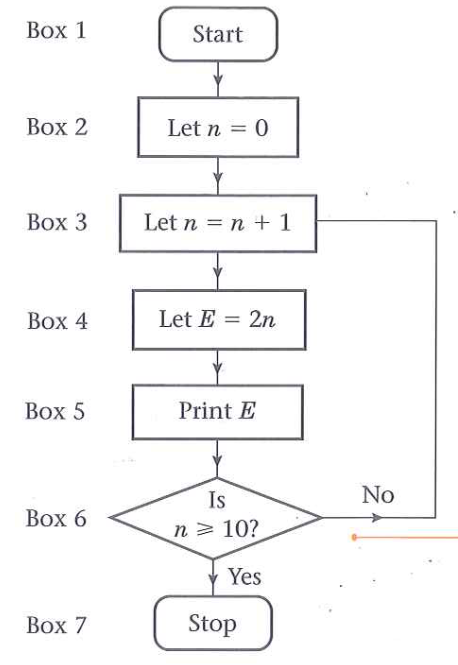
\includegraphics[scale=0.4]{img_D/1.png}
	\end{proof}

\end{eg}

\subsection{Bubble sort}
\subsection{Binary search}
\subsection{Implement the three bin packing algorithms}

\section{Graphs and networks}
\subsection{Basic Graph theory}
\begin{defi}[Vertices and Edges of Graph]
	In the graph G, above
	\begin{itemize}
		\item the vertices (or nodes) are:
		\item the edges (or arcs) are:
	\end{itemize}
\end{defi}

\begin{defi}[Subgraph]
	A subgraph of $G$ is a graph , each of whose vertices belongs to $G$ and each of whose edges belongs to $G$. It is simply a part of the original graph.
\end{defi}

\begin{defi}[Degree]
	The degree or valency or order of a vertex is the number of edges incident to it
\end{defi}

\begin{prop}
	If the degree of a vertex is even , we say it has even degree
\end{prop}

\begin{defi}[Path]
	A path is a finite sequence of edges, such that the end vertex of one edge in the sequence is the start vertex of the next, and in which no vertex appears more than once.
\end{defi}

\begin{defi}[Walk]
	A walk is a path in which you are permitted to return to vertices more than once.
\end{defi}

\begin{defi}[Cycle]
	A cycle is a closed 'path'.
\end{defi}
\begin{tikzpicture}

	\def \n {5}
	\def \radius {3cm}
	\def \margin {8} % margin in angles, depends on the radius

	\foreach \s in {1,...,\n}
	{
	\node[draw, circle] at ({360/\n * (\s - 1)}:\radius) {$\s$};
	\draw[->, >=latex] ({360/\n * (\s - 1)+\margin}:\radius)
	arc ({360/\n * (\s - 1)+\margin}:{360/\n * (\s)-\margin}:\radius);
	}
\end{tikzpicture}

\begin{defi}[Connected]
	Two vertices are connected if there is a path between them. A graph is connected if all its vertices are connected.
\end{defi}

\begin{defi}[Loop]
	A loop is an edge that starts and finishes at the same vertex
\end{defi}

\begin{defi}[Simple graph]
	A simple graph is one in which there are no loops and not have more than one edge connecting any pair of vertices
\end{defi}

\begin{defi}[Digraph]
	If the edges of a graph have a direction associated with them they are known as directed edges and the graph is known as a digraph.
\end{defi}

\begin{defi}[Tree]
	A tree is a connected graph with no cycles
\end{defi}

\begin{defi}[Spanning tree]
	A spanning tree of a graph ,$G$ is a subgraph which includes all the vertices of $G$ and is also a tree.
\end{defi}

\begin{defi}[Bipartite graph]
	A bipartite graph consists of two sets of vertices , $X$ and $Y$. The edges only join vertices in $X$ to vertices in $Y$, not vertices within a set
\end{defi}

\begin{tikzpicture}[thick,
		fsnode/.style={},
		ssnode/.style={},
		every fit/.style={ellipse,draw,inner sep=5pt,text width=2cm},
		->,shorten >= 3pt,shorten <= 3pt
	]

	% the vertices of U
	\begin{scope}[start chain=going below,node distance=7mm]
		\foreach \i/\xcoord/\ycoord in {1/6/8,2/5/1,3/-4/7,4/6/9,5/0/-3}
		\node[fsnode,on chain,label=left:$t_{\i}$] (f\i) {$(\xcoord,\ycoord)$};
	\end{scope}

	% the vertices of V
	\begin{scope}[xshift=4cm,yshift=-0.5cm,start chain=going below,node distance=7mm]
		\foreach \i/\xcoord/\ycoord in {6/0/3,7/1/4,8/-2/1,9/5/9}
		\node[ssnode,on chain,label=right:$t_{\i}$] (s\i) {$(\xcoord,\ycoord)$};
	\end{scope}

	% the set U
	\node [mblue,fit=(f1) (f5),label=above:$X$] {};
	% the set V
	\node [mgreen,fit=(s6) (s9),label=above:$Y$] {};

	% the edges
	\draw (f1) -- (s6);
	\draw (s6) -- (f2);
	\draw (f2) -- (s7);
	\draw (s7) -- (f3);
	\draw (s8) -- (f3);
	\draw (f3) -- (s9);
	\draw (s9) -- (f5);
	\draw (f5) -- (s6);
\end{tikzpicture}

\newpage

\begin{defi}[Complete graph]
	A complete graph is a graph in which every vertex is directly connected by an edge to each of the other vertices. If the graph has $n$ vertices the connected graph is denoted by $K_n$.
\end{defi}

\begin{tikzpicture}[transform shape,line width=0.2pt]
	\foreach \x in {1,...,16}{%
			\pgfmathparse{(\x-1)*45+floor(\x/9)*22.5}
			\node[draw,circle,inner sep=0.25cm] (N-\x) at (\pgfmathresult:5.4cm) [thick] {};
		}
	\foreach \x [count=\xi from 1] in {2,...,16}{%
			\foreach \y in {\x,...,16}{%
					\path (N-\xi) edge[-] (N-\y);
				}
		}
\end{tikzpicture}

\begin{defi}[Complete bipartite graph]
	A complete bipartite graph (denoted by $K_{r,s}$) in which there are $r$ vertices in set $X$ and $s$ vertices in set $Y$.
\end{defi}


\begin{defi}[Isomorphic graphs]
	Isomorphic graphs are graphs that who the same information but are drawn differently
\end{defi}

\subsection{Adjacency Matrix and Distance matrix}
\begin{defi}[Adjacency Matrix]
	A adjacency matrix records the number of direct links between vertices
\end{defi}

\begin{eg}
	Use an adjacency matrix to represent this graph\\

	\begin{tabular}{c|cccccc}
		  & A & B & C & D & E & F \\
		\hline
		A & 0 & 1 & 0 & 0 & 0 & 0 \\
		B & 1 & 0 & 1 & 0 & 2 & 1 \\
		C & 0 & 1 & 0 & 1 & 1 & 0 \\
		D & 0 & 0 & 1 & 0 & 0 & 1 \\
		E & 0 & 2 & 1 & 0 & 0 & 1 \\
		F & 0 & 1 & 0 & 1 & 1 & 2 \\
	\end{tabular}
	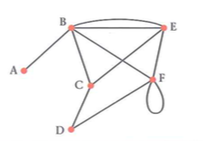
\includegraphics{img_D/2_2ex1}
\end{eg}


\begin{defi}[Distance Matrix]
	A distance matrix records the weights on the edges. Where there is no edge , we write '$-$'
\end{defi}
\begin{eg}
	Use a distance matrix to represent this network.\\
	\begin{tabular}{c|cccccc}
		  & A & B & C & D & E & F \\
		\hline
		A & 0 & 1 & 0 & 0 & 0 & 0 \\
		B & 1 & 0 & 1 & 0 & 2 & 1 \\
		C & 0 & 1 & 0 & 1 & 1 & 0 \\
		D & 0 & 0 & 1 & 0 & 0 & 1 \\
		E & 0 & 2 & 1 & 0 & 0 & 1 \\
		F & 0 & 1 & 0 & 1 & 1 & 2 \\
	\end{tabular}
	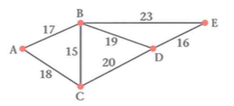
\includegraphics{img_D/2_2ex2}
\end{eg}
\begin{eg}
	Use a distance matrix to represent this directed network.\\
	\begin{tabular}{c|ccccc}
		  & A  & B  & C  & D  & E  \\
		\hline
		A & -  & 17 & 18 & -  & -  \\
		B & 17 & -  & 15 & 19 & 23 \\
		C & 18 & 15 & -  & 20 & -  \\
		D & -  & 19 & 20 & -  & 16 \\
		E & -  & 23 & -  & 16 & -  \\
	\end{tabular}
	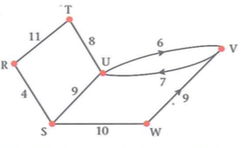
\includegraphics{img_D/2_2ex3}
\end{eg}
\section{Algorithms on networks}
\subsection{Kruskal's algorithm}
Kruskal's algorithm finds the shortest, cheapest or fastest way of linking all the nodes into one system\\
You can use Kruskal's algorithm to find a minimum spanning tree.
\begin{defi}[Minimum spanning tree]
	A minimum spanning tree (MST) is spanning tree such that the total length of its edges is as small as possible. (An MST is sometimes called a minimum connectors).
\end{defi}

\begin{defi}[Kruskal's algorithm]
	Here is Kruskal's algorithm.
	\begin{enumerate}
		\item Sort all the edges into ascending order of weight.
		\item Select the edges of least weight to start the tree
		\item Consider the next edge of least weight.\begin{itemize}
			      \item If it would form a cycle with the edges already selected, reject it. \item If it does not form a cycle, add it to the tree.
		      \end{itemize}
		      If there is choice of equal edges, consider each in turn.
		\item Repeat step 3 until all vertices are connected.
	\end{enumerate}

\end{defi}

\begin{eg}
	Use Kruskal's algorithm to find a minimum spanning tree
\end{eg}

\begin{eg}

\end{eg}

\subsection{Prim's algorithm}
Like Kruskal's algorithm, Prim's algorithm finds the minimum spanning tree, but it uses a different approach.
\begin{defi}[Prim's algorithm]
	Here is Prim's algorithm
	\begin{enumerate}
		\item Choose any vertex to start the tree.
		\item \begin{itemize}
			      \item Select an edges of least weight that joins a vertex that is already in the tree to a vertex that is not yet in the tree.
			      \item If there is a choice of edges of equal weight , choose randomly.
		      \end{itemize}
		\item Repeat Step 2 until all the vertices are connected.
	\end{enumerate}
\end{defi}

\begin{eg}

\end{eg}

You can apply Prim's algorithm to a distance matrix
\begin{defi}[Prim's algorithm to a distance matrix]
	Here is the distance matrix form of Prim's algorithm
	\begin{enumerate}
		\item Choose any vertex to start the tree.
		\item Delete the row in the matrix for the chosen vertex.
		\item Number the column in the matrix for the chosen vertex
		\item Put a ring round the lowest undeleted entry in the numbered columns. (If there is an equal choice, choose randomly.)
		\item The ringed entry becomes the nest edge to be added to the tree.
		\item Repeats steps 2,3,4 and 5 until all rows are deleted.
	\end{enumerate}
\end{defi}

\begin{eg}
	\begin{tabular}{c|ccccc}
	\end{tabular}
\end{eg}

\subsection{Dijkstra's algorithm}
Dijkstra's algorithm is used to find the shortest, cheapest or quickest route between two vertices.

\begin{defi}[Dijkstra's algorithm]
	Here is Dijkstra's algorithm\\
	(to find the shortest path form $S$ to $T$ through a network).
	\begin{enumerate}
		\item Label the start vertex , $S$ , with the final label ,$0$.
		\item Record a working value at every vertex , $Y$, that is directly connected to the vertex , $X$ , that has just received its final label.
		      \begin{itemize}
			      \item Working value at $Y=$ final value at $X+$ weight of arc $XY$
			      \item If there is already a working value at $Y$, it is only replaced if the new value is smaller.
			      \item Ince a vertex has a final label it is not revisited and its working values are no longer considered.
		      \end{itemize}
		\item Look at the working values at all vertices without final labels. Select the smallest working value. This now becomes the final label at that vertex. (If two vertices have the same smallest working  value either may be given its final label first.)
		\item Repeat steps 2 and 3 until the destination vertex , $T$, receives its final label.
		\item To find the shortest path, trace back from $T$ to $S$. Given that $B$ already lies on the route, include arc $AB$ whenever final label of $B$ - final label of $A$ $=$ weight of arc $AB$.
	\end{enumerate}
\end{defi}
\begin{eg}

\end{eg}
\begin{eg}

\end{eg}
\begin{eg}

\end{eg}

\section{Route inspection (Chinese postman problem)}

\subsection{Traversable}

\begin{defi}[Eulerian]
	If all the degrees in a graph are even, then the graph is Eulerian. If precisely two degrees are odd, and all the rest are even, then the graph is semi-Eulerian
\end{defi}

\begin{defi}[Traversable]
	A graph is traversable if it is possible to traverse (travel along) every arc just once without taking your pen from the paper.

\end{defi}

\begin{prop}
	A graph traversable if all the degrees are even
\end{prop}

\begin{prop}
	A graph is semi-traversable if it has precisely two odd degrees. In this case the start point and the finish point will be the two vertices with odd degrees.
\end{prop}

\begin{prop}
	A graph is not traversable if it has more than two odd degrees.
\end{prop}

\begin{eg}

\end{eg}

\begin{eg}

\end{eg}

\begin{eg}

\end{eg}

\subsection{Chinese postman algorithm (route inspection algorithm)}
You can use this algorithm to find the shortest route in a network that traverses every arc at least once and returns to the starting point.
\begin{prop}
	If all the vertices have even degree the network is traversable. The length of the shortest route will be equal to the weight of the network
\end{prop}
\begin{eg}

\end{eg}
\begin{prop}

\end{prop}
\begin{eg}

\end{eg}
\begin{eg}

\end{eg}

\begin{defi}[Route inspection algorithm]
	Here is the route inspection algorithm
	\begin{enumerate}
		\item Identify any vertices with odd degree.
		\item Consider all possible complete pairings of these vertices.
		\item Select the complete pairing that has the least sum.
		\item Add a repeat of the arcs indicated by this pairing to the network.
	\end{enumerate}
\end{defi}

\begin{eg}

\end{eg}


\section{Critical path analysis}
\subsection{Basic calculation}
\begin{eg}
	Draw an activity network using activity on arc for this precedence table. Use exactly two dummies.\\
	\begin{center}
		\begin{tabular}{|c|c|}
			\hline
			Activity & Immediately preceding activities \\
			\hline
			A        & -                                \\
			\hline
			B        & A                                \\
			\hline
			C        & A                                \\
			\hline
			D        & A                                \\
			\hline
			E        & B                                \\
			\hline
			F        & B,C                              \\
			\hline
			G        & D,F                              \\
			\hline
			H        & D                                \\
			\hline
			I        & G,H                              \\
			\hline
		\end{tabular}
	\end{center}
	\begin{center}
		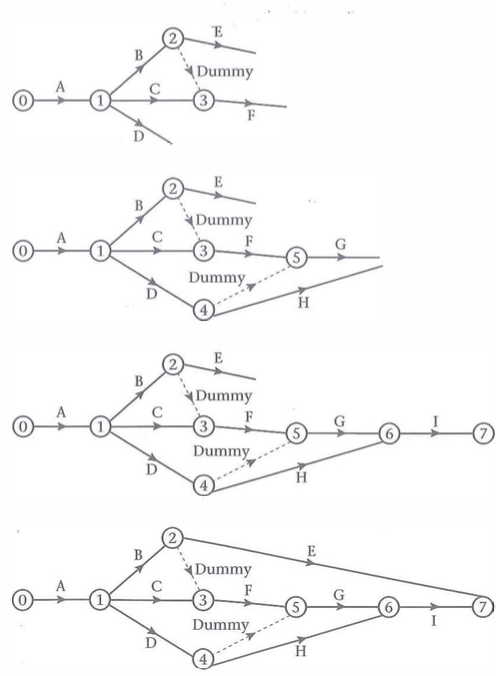
\includegraphics[scale=0.5]{img_D/5_4}
	\end{center}
\end{eg}

\newpage
\begin{eg}
	The diagram shows part of an activity network. Calculate the value of $x$.
	\begin{center}
		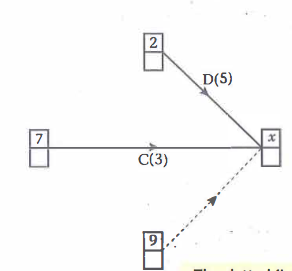
\includegraphics[scale=0.5]{img_D/5_5}
	\end{center}
	\begin{align*}
		2+5 & =7  \\
		7+3 & =10 \\
		9+0 & =9  \\
	\end{align*}
	The largest is 10, so $x=10$
\end{eg}

\begin{eg}
	The diagram shows part of an activity network. Calculate the value of $y$.
	\begin{center}
		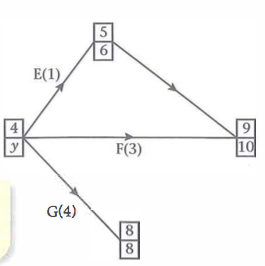
\includegraphics[scale=0.5]{img_D/5_6}
	\end{center}
	\begin{align*}
		6-1  & =5 \\
		10-3 & =7 \\
		8-4  & =4 \\
	\end{align*}
	The smallest is 4, so $y=4$
\end{eg}

\begin{defi}[Critical activity and path]
	The path(s) and node(s) which are directed to the results
\end{defi}

\subsection{Total float}
\begin{defi}[Total float]
	The total float of an activity is the amount of time that its start may be delayed without affecting the duration of the project.
	\[
		\text{total float}=\text{latest finish time}-\text{duration}-\text{earliest start time}
	\]
\end{defi}
\begin{eg}
	Determine the total float of each activity in this activity network.

	\begin{center}
		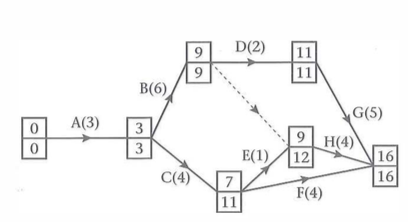
\includegraphics[scale=0.5]{img_D/5_10}
	\end{center}
	\begin{center}
		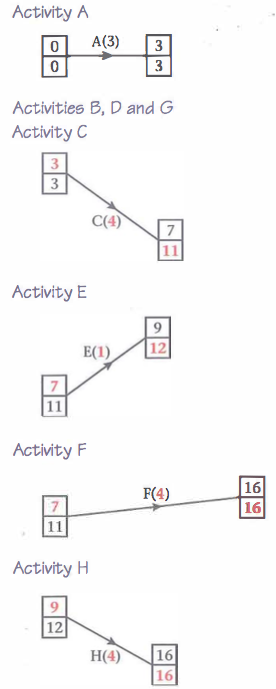
\includegraphics[scale=0.5]{img_D/5_10_1}
	\end{center}
	At Activity A, Any delay in the start time will affect the duration of the project. Total float $= 0$.\\
	C :  $11-4-3=4$\\
	E :  $12-1-7=4$\\
	F : $16-4-7=5$\\
	H :  $16-4-9=3$\\
\end{eg}

\begin{eg}
	Examples 11-14
\end{eg}

\subsection{Cascade (Gantt) charts}


\section{Linear programming}
\begin{center}
	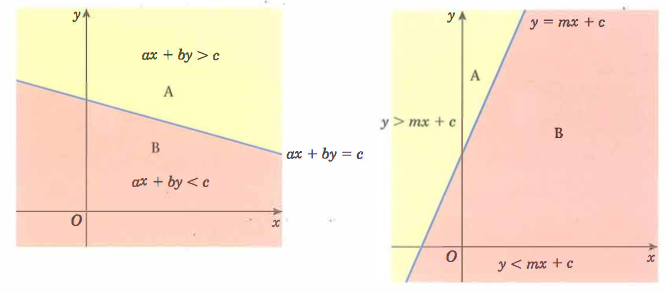
\includegraphics[scale=0.5]{img_D/6_intro}
\end{center}
\begin{remark}
	Using dotted line if the inequalities are $>$ or $<$
\end{remark}
\begin{eg}
	Example 5-13
\end{eg}


\section{Matchings}

\begin{eg}
	Example 3-6
\end{eg}

\section{Transportation problems}
\subsection{North-west corner method}
\begin{eg}
	Use the north-west corner method to find an initial solution to the problem described in that example and shown in the table
	\begin{center}
		\begin{tabular}{|c|c|c|c|c|c|}
			\hline
			           & Depot W & Depot X & Depot Y & Depot Z & Stock \\
			\hline
			Supplier A & 180     & 110     & 130     & 290     & 14    \\
			\hline
			Supplier B & 190     & 250     & 150     & 280     & 16    \\
			\hline
			Supplier C & 240     & 270     & 190     & 120     & 20    \\
			\hline
			Demand     & 11      & 15      & 14      & 10      & 50    \\
			\hline
		\end{tabular}
	\end{center}
	\begin{proof}
		Set up the table
		\begin{center}
			\begin{tabular}{|c|c|c|c|c|c|}
				\hline
				           & Depot W & Depot X & Depot Y & Depot Z & Stock \\
				\hline
				Supplier A &         &         &         &         & 14    \\
				\hline
				Supplier B &         &         &         &         & 16    \\
				\hline
				Supplier C &         &         &         &         & 20    \\
				\hline
				Demand     & 11      & 15      & 14      & 10      & 50    \\
				\hline
			\end{tabular}
		\end{center}
		Look at the column demand first which is lowest, write down the value on left top corner
		\begin{center}
			\begin{tabular}{|c|c|c|c|c|c|}
				\hline
				           & Depot W & Depot X & Depot Y & Depot Z & Stock \\
				\hline
				Supplier A & 11      &         &         &         & 14    \\
				\hline
				Supplier B &         &         &         &         & 16    \\
				\hline
				Supplier C &         &         &         &         & 20    \\
				\hline
				Demand     & 11      & 15      & 14      & 10      & 50    \\
				\hline
			\end{tabular}
		\end{center}
		write down the different between the row and you previous number on right
		\begin{center}
			\begin{tabular}{|c|c|c|c|c|c|}
				\hline
				           & Depot W & Depot X & Depot Y & Depot Z & Stock \\
				\hline
				Supplier A & 11      & 3       &         &         & 14    \\
				\hline
				Supplier B &         &         &         &         & 16    \\
				\hline
				Supplier C &         &         &         &         & 20    \\
				\hline
				Demand     & 11      & 15      & 14      & 10      & 50    \\
				\hline
			\end{tabular}
		\end{center}
		write down the different between the column and you previous number on below

		\begin{center}
			\begin{tabular}{|c|c|c|c|c|c|}
				\hline
				           & Depot W & Depot X & Depot Y & Depot Z & Stock \\
				\hline
				Supplier A & 11      & 3       &         &         & 14    \\
				\hline
				Supplier B &         & 12      &         &         & 16    \\
				\hline
				Supplier C &         &         &         &         & 20    \\
				\hline
				Demand     & 11      & 15      & 14      & 10      & 50    \\
				\hline
			\end{tabular}
		\end{center}
		write down the different between the row and you previous number on right
		\begin{center}
			\begin{tabular}{|c|c|c|c|c|c|}
				\hline
				           & Depot W & Depot X & Depot Y & Depot Z & Stock \\
				\hline
				Supplier A & 11      & 3       &         &         & 14    \\
				\hline
				Supplier B &         & 12      & 4       &         & 16    \\
				\hline
				Supplier C &         &         &         &         & 20    \\
				\hline
				Demand     & 11      & 15      & 14      & 10      & 50    \\
				\hline
			\end{tabular}
		\end{center}
		write down the different between the column and you previous number on below
		\begin{center}
			\begin{tabular}{|c|c|c|c|c|c|}
				\hline
				           & Depot W & Depot X & Depot Y & Depot Z & Stock \\
				\hline
				Supplier A & 11      & 3       &         &         & 14    \\
				\hline
				Supplier B &         & 12      & 4       &         & 16    \\
				\hline
				Supplier C &         &         & 10      &         & 20    \\
				\hline
				Demand     & 11      & 15      & 14      & 10      & 50    \\
				\hline
			\end{tabular}
		\end{center}
		write down the different between the row and you previous number on right
		\begin{center}
			\begin{tabular}{|c|c|c|c|c|c|}
				\hline
				           & Depot W & Depot X & Depot Y & Depot Z & Stock \\
				\hline
				Supplier A & 11      & 3       &         &         & 14    \\
				\hline
				Supplier B &         & 12      & 4       &         & 16    \\
				\hline
				Supplier C &         &         & 10      & 10      & 20    \\
				\hline
				Demand     & 11      & 15      & 14      & 10      & 50    \\
				\hline
			\end{tabular}
		\end{center}
		This is the final table. All of the stock has been used and all of the demands met.\\

		The number of occupied cells (routes used) in the table $=$ number of supply points $+$ number of demand points $-$ 1 .\\
		In this case the \\
		number of occupied cells (routes used) $= 6$, \\
		number of supply points $= 3$,\\
		number of demand points $= 4$ \\
		and $6 = 3 + 4 - 1$.\\

		Use this table, together with the table showing costs, to work out the total cost of the solution.
		\begin{center}
			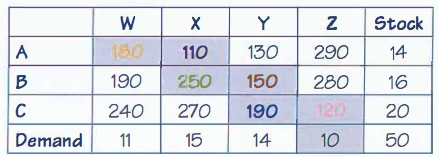
\includegraphics[scale=0.5]{img_D/8_2}
		\end{center}

		The total cost of this solution is $(11\times 180)+(3\times 110)+(12\times 250)+(4\times 150)+(10\times 190)+(10\times 120)=9010$
	\end{proof}
\end{eg}

\newpage
\begin{defi}[balanced]
	When the total supply $>$ total demand , we say the problem is unbalanced, If the problem is unbalanced we simply add a dummy demand point with a demand chosen so that total supply $=$ total demand, with transportation costs of zero.
\end{defi}
\begin{eg}
	Three outlets A, B and C are supplied by three suppliers X, Y and Z. The table shows the cost, in pounds, of transporting each unit, the number of units required at each outlet and the number of units available at each supplier.
	\begin{center}
		\begin{tabular}{|c|c|c|c|c|}
			\hline
			       & A  & B  & C  & Supply \\
			\hline
			X      & 9  & 11 & 10 & 40     \\
			\hline
			Y      & 10 & 8  & 12 & 60     \\
			\hline
			Z      & 12 & 7  & 8  & 50     \\
			\hline
			Demand & 50 & 40 & 30 &        \\
			\hline
		\end{tabular}
	\end{center}
	Add a dummy demand point and appropriate costs to the table.
	and use the north-west corner method to obtain an initial solution.

	\begin{proof}
		Here you are
		\begin{center}
			\begin{tabular}{|c|c|c|c|c|c|}
				\hline
				       & A  & B  & C  & D  & Supply \\
				\hline
				X      & 9  & 11 & 10 & 0  & 40     \\
				\hline
				Y      & 10 & 8  & 12 & 0  & 60     \\
				\hline
				Z      & 12 & 7  & 8  & 0  & 50     \\
				\hline
				Demand & 50 & 40 & 30 & 30 & 150    \\
				\hline
			\end{tabular}
		\end{center}

		\begin{center}
			\begin{tabular}{|c|c|c|c|c|c|}
				\hline
				       & A  & B  & C  & D  & Supply \\
				\hline
				X      & 40 &    &    &    & 40     \\
				\hline
				Y      & 10 & 40 & 10 &    & 60     \\
				\hline
				Z      &    &    & 20 & 30 & 50     \\
				\hline
				Demand & 50 & 40 & 30 & 30 & 150    \\
				\hline
			\end{tabular}
		\end{center}
	\end{proof}
\end{eg}

\begin{defi}[degenerate]
	In a feasible solution to a transportation problem with $m$ rows and $n$ columns, if the number
	of cells used is less than $n+m-1$, then the solution is degenerate
\end{defi}
\begin{eg}
	\begin{enumerate}
		\item Demonstrate that the north-west corner method gives a degenerate solution and explain why it is degenerate
		\item Adapt your solution to give a non-degenerate initial solution and state its cost.
	\end{enumerate}
	\begin{center}
		\begin{tabular}{|c|c|c|c|c|}
			\hline
			       & A  & B  & C  & Supply \\
			\hline
			W      & 10 & 11 & 6  & 30     \\
			\hline
			X      & 4  & 5  & 9  & 20     \\
			\hline
			Y      & 3  & 8  & 7  & 35     \\
			\hline
			Z      & 11 & 10 & 9  & 35     \\
			\hline
			Demand & 30 & 40 & 50 & 120    \\
			\hline
		\end{tabular}
	\end{center}
	\begin{proof}
		(i)
		\begin{center}
			\begin{tabular}{|c|c|c|c|c|}
				\hline
				       & A  & B  & C  & Supply \\
				\hline
				W      & 30 &    &    & 30     \\
				\hline
				X      &    & 20 &    & 20     \\
				\hline
				Y      &    & 20 & 15 & 35     \\
				\hline
				Z      &    &    & 35 & 35     \\
				\hline
				Demand & 30 & 40 & 50 & 120    \\
				\hline
			\end{tabular}
		\end{center}
		This solution is degenerate since it fulfils all the supply and demand needs but only uses 5 cells WA, XB, YB, YC and ZC. There are 4 rows and 3 columns so a non-degenerate solution will use $4+3-1=6$ cells.\\

		(ii)\\
		Start by placing the largest possible number in the north-west corner.

		\begin{center}
			\begin{tabular}{|c|c|c|c|c|}
				\hline
				       & A  & B  & C  & Supply \\
				\hline
				W      & 30 &    &    & 30     \\
				\hline
				X      &    &    &    & 20     \\
				\hline
				Y      &    &    &    & 35     \\
				\hline
				Z      &    &    &    & 35     \\
				\hline
				Demand & 30 & 40 & 50 & 120    \\
				\hline
			\end{tabular}
		\end{center}
		There are two possible initial solutions, depending on where you chose to place the zero\\

		either
		\begin{center}
			\begin{tabular}{|c|c|c|c|c|}
				\hline
				       & A  & B  & C  & Supply \\
				\hline
				W      & 30 &    &    & 30     \\
				\hline
				X      & 0  & 20 &    & 20     \\
				\hline
				Y      &    & 20 & 15 & 35     \\
				\hline
				Z      &    &    & 35 & 35     \\
				\hline
				Demand & 30 & 40 & 50 & 120    \\
				\hline
			\end{tabular}
		\end{center}
		Or
		\begin{center}
			\begin{tabular}{|c|c|c|c|c|}
				\hline
				       & A  & B  & C  & Supply \\
				\hline
				W      & 30 &    &    & 30     \\
				\hline
				X      & 0  & 20 &    & 20     \\
				\hline
				Y      &    & 20 & 15 & 35     \\
				\hline
				Z      &    &    & 35 & 35     \\
				\hline
				Demand & 30 & 40 & 50 & 120    \\
				\hline
			\end{tabular}
		\end{center}
	\end{proof}
\end{eg}
\subsection{Shadow costs}
\begin{defi}
	The sum of shadow costs of column and row equation to that overlaping number box
\end{defi}
\begin{eg}
	Calculate the shadow costs given by the initial solution.
	\begin{center}
		\begin{tabular}{|c|c|c|c|c|c|}
			\hline
			       & W   & X   & Y   & Z   & Stock \\
			\hline
			A      & 180 & 110 & 130 & 290 & 14    \\
			\hline
			B      & 190 & 250 & 150 & 280 & 16    \\
			\hline
			C      & 240 & 270 & 190 & 120 & 20    \\
			\hline
			Demand & 11  & 15  & 14  & 10  & 50    \\
			\hline
		\end{tabular}
	\end{center}
	\begin{proof}
		Initial solution was
		\begin{center}
			\begin{tabular}{|c|c|c|c|c|c|}
				\hline
				       & W  & X  & Y  & Z  & Stock \\
				\hline
				A      & 11 & 3  &    &    & 14    \\
				\hline
				B      &    & 12 & 4  &    & 16    \\
				\hline
				C      &    &    & 10 & 10 & 20    \\
				\hline
				Demand & 11 & 15 & 14 & 10 & 50    \\
				\hline
			\end{tabular}
		\end{center}
		Focus on the costs of the routes being used - the non-empty squares
		\begin{center}
			\begin{tabular}{|c|c|c|c|c|c|}
				\hline
				       & W   & X   & Y   & Z   & Stock \\
				\hline
				A      & 180 & 110 &     &     & 14    \\
				\hline
				B      &     & 250 & 150 &     & 16    \\
				\hline
				C      &     &     & 190 & 120 & 20    \\
				\hline
				Demand & 11  & 15  & 14  & 10  & 50    \\
				\hline
			\end{tabular}
		\end{center}
		Putting $S(A)=0$, from row 1 we get $D(W)=180$ and $D(X)=110$\\
		the solve the equations \\
		$S(A)+D(W)=180$\\
		$S(A)+D(X)=150$

		\begin{center}
			\begin{tabular}{|c|c|c|c|c|c|c|}
				\hline
				Shadow costs &            & 180     & 110     &         &         &       \\
				\hline
				             &            & Depot W & Depot X & Depot Y & Depot Z & Stock \\
				\hline
				0            & Supplier A & 180     & 110     &         &         & 14    \\
				\hline
				             & Supplier B &         & 250     & 150     &         & 16    \\
				\hline
				             & Supplier C &         &         & 190     & 120     & 20    \\
				\hline
				             & Demand     & 11      & 15      & 14      & 10      & 50    \\
				\hline
			\end{tabular}
		\end{center}
		Now move to Row 2. \\
		You know that $D(X)=110$, so you find $S(B)=140$ \\
		hence $D(Y)=10$
		\begin{center}
			\begin{tabular}{|c|c|c|c|c|c|c|}
				\hline
				Shadow costs &            & 180     & 110     & 10      &         &       \\
				\hline
				             &            & Depot W & Depot X & Depot Y & Depot Z & Stock \\
				\hline
				0            & Supplier A & 180     & 110     &         &         & 14    \\
				\hline
				140          & Supplier B &         & 250     & 150     &         & 16    \\
				\hline
				             & Supplier C &         &         & 190     & 120     & 20    \\
				\hline
				             & Demand     & 11      & 15      & 14      & 10      & 50    \\
				\hline
			\end{tabular}
		\end{center}
		Move to Row 3 \\
		You know that $D(Y)=10$ , so we find \\
		$S(C) = 180$ and hence that $D(Z)=-60$
		\begin{center}
			\begin{tabular}{|c|c|c|c|c|c|c|}
				\hline
				Shadow costs &            & 180     & 110     & 10      & -60     &       \\
				\hline
				             &            & Depot W & Depot X & Depot Y & Depot Z & Stock \\
				\hline
				0            & Supplier A & 180     & 110     &         &         & 14    \\
				\hline
				140          & Supplier B &         & 250     & 150     &         & 16    \\
				\hline
				160          & Supplier C &         &         & 190     & 120     & 20    \\
				\hline
				             & Demand     & 11      & 15      & 14      & 10      & 50    \\
				\hline
			\end{tabular}
		\end{center}
		Done.
	\end{proof}
\end{eg}


\begin{eg}
	Calculate the shadow costs given by the initial solution.
	\begin{center}
		\begin{tabular}{|c|c|c|c|c|}
			\hline
			       & A  & B  & C  & Supply \\
			\hline
			X      & 9  & 11 & 10 & 40     \\
			\hline
			Y      & 10 & 8  & 12 & 60     \\
			\hline
			Z      & 12 & 7  & 8  & 50     \\
			\hline
			Demand & 50 & 40 & 30 &        \\
			\hline
		\end{tabular}
	\end{center}
	Add a dummy demand point and appropriate costs to the table.
	and use the north-west corner method to obtain an initial solution.

	\begin{proof}
		Here you are
		\begin{center}
			\begin{tabular}{|c|c|c|c|c|c|}
				\hline
				       & A  & B  & C  & D  & Supply \\
				\hline
				X      & 9  & 11 & 10 & 0  & 40     \\
				\hline
				Y      & 10 & 8  & 12 & 0  & 60     \\
				\hline
				Z      & 12 & 7  & 8  & 0  & 50     \\
				\hline
				Demand & 50 & 40 & 30 & 30 & 150    \\
				\hline
			\end{tabular}
		\end{center}
		\begin{center}
			\begin{tabular}{|c|c|c|c|c|c|}
				\hline
				       & A  & B  & C  & D  & Supply \\
				\hline
				X      & 40 &    &    &    & 40     \\
				\hline
				Y      & 10 & 40 & 10 &    & 60     \\
				\hline
				Z      &    &    & 20 & 30 & 50     \\
				\hline
				Demand & 50 & 40 & 30 & 30 & 150    \\
				\hline
			\end{tabular}
		\end{center}
		\begin{center}
			\begin{tabular}{|c|c|c|c|c|c|c|}
				\hline
				Shadow costs &        & 9  & 7  & 11 & 3  &        \\
				\hline
				             &        & A  & B  & C  & D  & Supply \\
				\hline
				0            & X      & 40 &    &    &    & 40     \\
				\hline
				1            & Y      & 10 & 40 & 10 &    & 60     \\
				\hline
				-3           & Z      &    &    & 20 & 30 & 50     \\
				\hline
				             & Demand & 50 & 40 & 30 & 30 & 150    \\
				\hline
			\end{tabular}
		\end{center}
	\end{proof}
\end{eg}
\subsection{Improvement indices}
\begin{defi}[Improvement index]
	The improvement index in sending a unit from a source P to a demand point Q is found by subtracting the source cost $S(P)$ and destination cost $D(Q)$ from the stated cost of transporting one unit along that route $C(PQ)$. i.e.
	\[
		\text{Improvement index for PQ}=I_{PQ}=C(PQ)-S(P)-D(Q)
	\]
\end{defi}
\begin{defi}[Optimal]
	If there are no negative improvement indices.
\end{defi}
\begin{eg}
	Calculate the improvement indices
	\begin{center}
		\begin{tabular}{|c|c|c|c|c|c|c|}
			\hline
			Shadow costs &            & 180     & 110     & 10      & -60     &       \\
			\hline
			             &            & Depot W & Depot X & Depot Y & Depot Z & Stock \\
			\hline
			0            & Supplier A & 180     & 110     &         &         & 14    \\
			\hline
			140          & Supplier B &         & 250     & 150     &         & 16    \\
			\hline
			160          & Supplier C &         &         & 190     & 120     & 20    \\
			\hline
			             & Demand     & 11      & 15      & 14      & 10      & 50    \\
			\hline
		\end{tabular}
	\end{center}
	$BW=-130$\\
	$CW=-120$\\
	$ CX=-20$\\
	$ AY=120$\\
	$ AZ=350$\\
	$ BZ=200$\\
\end{eg}


\subsection{Stepping-stone method}

\begin{eg}
	Obtain an improved solution and find the improved cost.
	\begin{center}
		\begin{tabular}{|c|c|c|c|c|c|}
			\hline
			           & Depot W & Depot X & Depot Y & Depot Z & Stock \\
			\hline
			Supplier A & 180     & 110     & 130     & 290     & 14    \\
			\hline
			Supplier B & 190     & 250     & 150     & 280     & 16    \\
			\hline
			Supplier C & 240     & 270     & 190     & 120     & 20    \\
			\hline
			Demand     & 11      & 15      & 14      & 10      & 50    \\
			\hline
		\end{tabular}
	\end{center}
	and the initial solution was
	\begin{center}
		\begin{tabular}{|c|c|c|c|c|c|}
			\hline
			           & Depot W & Depot X & Depot Y & Depot Z & Stock \\
			\hline
			Supplier A & 11      & 3       &         &         & 14    \\
			\hline
			Supplier B &         & 12      & 4       &         & 16    \\
			\hline
			Supplier C &         &         & 10      & 10      & 20    \\
			\hline
			Demand     & 11      & 15      & 14      & 10      & 50    \\
			\hline
		\end{tabular}
	\end{center}
	at a cost of 9010
	\begin{proof}
		Use BW as the entering cell, since this gave the most negative improvement index, -130. So BW will be and increasing cell. We enter a value of $\theta$ into this cell
		\begin{center}
			\begin{tabular}{|c|c|c|c|c|c|}
				\hline
				           & Depot W  & Depot X & Depot Y & Depot Z & Stock \\
				\hline
				Supplier A & 11       & 3       &         &         & 14    \\
				\hline
				Supplier B & $\theta$ & 12      & 4       &         & 16    \\
				\hline
				Supplier C &          &         & 10      & 10      & 20    \\
				\hline
				Demand     & 11       & 15      & 14      & 10      & 50    \\
				\hline
			\end{tabular}
		\end{center}
		In order to keep the demand at W correct. you must therefore decrease the entry at AW, so AW will be a decreasing cell
		\begin{center}
			\begin{tabular}{|c|c|c|c|c|c|}
				\hline
				           & Depot W     & Depot X & Depot Y & Depot Z & Stock \\
				\hline
				Supplier A & 11$-\theta$ & 3       &         &         & 14    \\
				\hline
				Supplier B & $\theta$    & 12      & 4       &         & 16    \\
				\hline
				Supplier C &             &         & 10      & 10      & 20    \\
				\hline
				Demand     & 11          & 15      & 14      & 10      & 50    \\
				\hline
			\end{tabular}
		\end{center}
		In order to keep the demand at A correct. you must therefore decrease the entry at AX, so AW will be a increasing cell
		\begin{center}
			\begin{tabular}{|c|c|c|c|c|c|}
				\hline
				           & Depot W     & Depot X    & Depot Y & Depot Z & Stock \\
				\hline
				Supplier A & 11$-\theta$ & 3$+\theta$ &         &         & 14    \\
				\hline
				Supplier B & $\theta$    & 12         & 4       &         & 16    \\
				\hline
				Supplier C &             &            & 10      & 10      & 20    \\
				\hline
				Demand     & 11          & 15         & 14      & 10      & 50    \\
				\hline
			\end{tabular}
		\end{center}
		In order to keep the demand at X correct. you must therefore decrease the entry at BX, so BX will be a decreasing cell
		\begin{center}
			\begin{tabular}{|c|c|c|c|c|c|}
				\hline
				           & Depot W     & Depot X     & Depot Y & Depot Z & Stock \\
				\hline
				Supplier A & 11$-\theta$ & 3$+\theta$  &         &         & 14    \\
				\hline
				Supplier B & $\theta$    & 12$-\theta$ & 4       &         & 16    \\
				\hline
				Supplier C &             &             & 10      & 10      & 20    \\
				\hline
				Demand     & 11          & 15          & 14      & 10      & 50    \\
				\hline
			\end{tabular}
		\end{center}
		Now choose a value for $\theta$, the greatest value you can, without intoducing negative entries into the table. Look at the decreasing cells and see that the greatest value of $\theta$ is 11 (since $11-11=0$)\\

		Replace $\theta$ by 11 in the table
		\begin{center}
			\begin{tabular}{|c|c|c|c|c|c|}
				\hline
				           & Depot W & Depot X & Depot Y & Depot Z & Stock \\
				\hline
				Supplier A & 11$-11$ & 3$+11$  &         &         & 14    \\
				\hline
				Supplier B & $11$    & 12$-11$ & 4       &         & 16    \\
				\hline
				Supplier C &         &         & 10      & 10      & 20    \\
				\hline
				Demand     & 11      & 15      & 14      & 10      & 50    \\
				\hline
			\end{tabular}
		\end{center}
		This gives the improved solution:
		\begin{center}
			\begin{tabular}{|c|c|c|c|c|c|}
				\hline
				           & Depot W & Depot X & Depot Y & Depot Z & Stock \\
				\hline
				Supplier A &         & 14      &         &         & 14    \\
				\hline
				Supplier B & $11$    & 1       & 4       &         & 16    \\
				\hline
				Supplier C &         &         & 10      & 10      & 20    \\
				\hline
				Demand     & 11      & 15      & 14      & 10      & 50    \\
				\hline
			\end{tabular}
		\end{center}
		this solution has a cost of 7580\\

		As a double check, it is always true that
		\[
			\text{New cost}=\text{cost of former solution}+\text{improvement index}\times\theta
		\]
		In this case $7580=9010+(-130\times 11)$

		You will notice that AW has become empty that is exiting cell
	\end{proof}
\end{eg}

\begin{eg}
	We also find an optimal solution\\
	\begin{proof}
		Second iteration\\
		The improvement indices are:\\
		$AW=130$\\
		$CW=10$\\
		$CX=-20$\\
		$AY=120$\\
		$AZ=350$\\
		$BZ=200$\\

		So the new entering cell is CX, since this has the most negative improvement index \\

		Applying the stepping-stone method gives
		\begin{center}
			\begin{tabular}{|c|c|c|c|c|c|}
				\hline
				           & Depot W & Depot X    & Depot Y       & Depot Z & Stock \\
				\hline
				Supplier A &         & 14         &               &         & 14    \\
				\hline
				Supplier B & $11$    & 1$-\theta$ & 4$+\theta$    &         & 16    \\
				\hline
				Supplier C &         & $\theta$   & 10  $-\theta$ & 10      & 20    \\
				\hline
				Demand     & 11      & 15         & 14            & 10      & 50    \\
				\hline
			\end{tabular}
		\end{center}
		Looking at cells BX and CY we see that the greatest value for $\theta$ is 1\\

		The new exiting cell will be BX, $\theta=1$ and we get
		\begin{center}
			\begin{tabular}{|c|c|c|c|c|c|}
				\hline
				           & Depot W & Depot X & Depot Y & Depot Z & Stock \\
				\hline
				Supplier A &         & 14      &         &         & 14    \\
				\hline
				Supplier B & $11$    &         & 5       &         & 16    \\
				\hline
				Supplier C &         & 1       & 9       & 10      & 20    \\
				\hline
				Demand     & 11      & 15      & 14      & 10      & 50    \\
				\hline
			\end{tabular}
		\end{center}
		The new cost is 7560\\

		Checking $7580+(-20)\times 1=7560$\\

		Third iteration
		\begin{center}
			\begin{tabular}{|c|c|c|c|c|c|c|c|}
				\hline
				Shadow costs &        & 70  & 110 & 30  & -40 &       \\
				\hline
				             &        & W   & X   & Y   & Z   & Stock \\
				\hline
				0            & A      & 180 & 110 & 130 & 290 & 14    \\
				\hline
				120          & B      & 190 & 250 & 150 & 180 & 16    \\
				\hline
				160          & C      & 240 & 270 & 190 & 120 & 20    \\
				\hline
				             & Demand & 11  & 15  & 14  & 10  & 50    \\
				\hline
			\end{tabular}
		\end{center}
		There are no negative improvement indices so this solution is optimal (by Calculate the improvement indices)
	\end{proof}

\end{eg}
\subsection{Transportation problem and linear programming}
\begin{eg}
	Formulate the transportation problem as a linear programming problem. You must state your decision variables, objective and constraints.
	\begin{center}
		\begin{tabular}{c|c|c|c|c}
			       & R  & S  & T  & Supply \\
			\hline
			A      & 3  & 3  & 2  & 25     \\
			\hline
			B      & 4  & 2  & 3  & 40     \\
			\hline
			C      & 3  & 4  & 3  & 31     \\
			\hline
			Demand & 30 & 30 & 36 &        \\
		\end{tabular}
	\end{center}
	\begin{proof}
		Let $x_{ij}$ be the number of units transported from $i$ to $j$\\
		where $i\in \{A,B,C\}$ and $J\in \{R,S,T\}$ and $x_{ij}\geq 0$\\
		\begin{align*}
			\text{Minimise} C & =3x_{11}+3x_{12}+2x_{13} \\
			                  & +4x_{21}+2x_{22}+3x{23}  \\
			                  & +3x_{31}+4x_{32}+3x_{33}
		\end{align*}
		Subject to:
		\begin{align*}
			x_{11}+x_{12}+x_{13} & \leq 25 \\
			x_{21}+x_{22}+x_{23} & \leq 40 \\
			x_{31}+x_{32}+x_{33} & \leq 31 \\
			x_{11}+x_{21}+x_{31} & \leq 30 \\
			x_{12}+x_{22}+x_{32} & \leq 30 \\
			x_{13}+x_{23}+x_{33} & \leq 36 \\
		\end{align*}
	\end{proof}
\end{eg}

\section{Allocation (assignment) problems}
\subsection{Reduce cost matrics}
To subtract the least value for each element of that row and then column repeatlly.
\begin{eg}
  Reduce the cost matrix
	\begin{center}
		\begin{tabular}{|c|c|c|c|c|}
			\hline
			      & Task W & Task X & Task Y & Task Z \\
			\hline
			Kris  & 12     & 23     & 15     & 40     \\
			\hline
			Laura & 14     & 21     & 17     & 20     \\
			\hline
			Sam   & 13     & 22     & 20     & 30     \\
			\hline
			Steve & 14     & 24     & 13     & 10     \\
			\hline
		\end{tabular}
  \end{center}
  \begin{proof}
   reduce the least number of the row of each row
    \begin{center}
      \begin{tabular}{|c|c|c|c|c|}
        \hline
              & Task W & Task X & Task Y & Task Z \\
        \hline
        Kris  & 0     & 11     & 3     & 28     \\
        \hline
        Laura & 0     & 7     & 3     & 6     \\
        \hline
        Sam   & 0     & 9     & 7     & 17     \\
        \hline
        Steve & 4     & 14     & 3     & 0     \\
        \hline
      \end{tabular}
    \end{center}
    reduce the least number of the column of each column
    \begin{center}
      \begin{tabular}{|c|c|c|c|c|}
        \hline
              & Task W & Task X & Task Y & Task Z \\
        \hline
        Kris  & 0     & 4     & 0     & 28     \\
        \hline
        Laura & 0     & 0     & 0     & 6     \\
        \hline
        Sam   & 0     & 2     & 4     & 17     \\
        \hline
        Steve & 4     & 7     & 0     & 0     \\
        \hline
      \end{tabular}
    \end{center}
    If we can find a matching using only the cells showing a zero cost we will have found an optimal solution. In this case we can.\\
    
    Oue optimal solution is\\
    
    Kris does task Y Laura does task X Sam does task W and Steve does task Z\\
    
    If you look at the original cost matrix the total cost is $15+21+13+10=59$\\
    
    Check total cost was 59 which is also the value of all the row and column reductions we made $(12+14+13+10+7+3=59)$

  \end{proof}
  
\end{eg}
\subsection{Hungarian algorithm}
\begin{enumerate}
  \item 
  \item 
  \item 
  \item 
  \item 
  \item 
  \item 
\end{enumerate}
\begin{eg}
  2-9
\end{eg}

\section{The travelling salesman problem}
\begin{eg}
  example 2-10
\end{eg}

\section{Further linear programming}
\begin{eg}
1-13
\end{eg}

\section{Game theory}
\begin{eg}
  1-12
  \end{eg}

\section{Network flows}
\begin{eg}
  1-16
  \end{eg}

\section{Dynamic programming}

\begin{eg}
  1-10
  \end{eg}

\end{document}